\hypertarget{Personne_8cpp}{}\section{Personne.\+cpp File Reference}
\label{Personne_8cpp}\index{Personne.\+cpp@{Personne.\+cpp}}


Cette classe sert au maintien et à la manipulation des personnes. Cette classe est abstraite.  


{\ttfamily \#include \char`\"{}Date.\+h\char`\"{}}\newline
{\ttfamily \#include \char`\"{}Personne.\+h\char`\"{}}\newline
{\ttfamily \#include \char`\"{}validation\+Format.\+h\char`\"{}}\newline
{\ttfamily \#include \char`\"{}Contrat\+Exception.\+h\char`\"{}}\newline
{\ttfamily \#include $<$sstream$>$}\newline
{\ttfamily \#include $<$iomanip$>$}\newline
Include dependency graph for Personne.\+cpp\+:\nopagebreak
\begin{figure}[H]
\begin{center}
\leavevmode
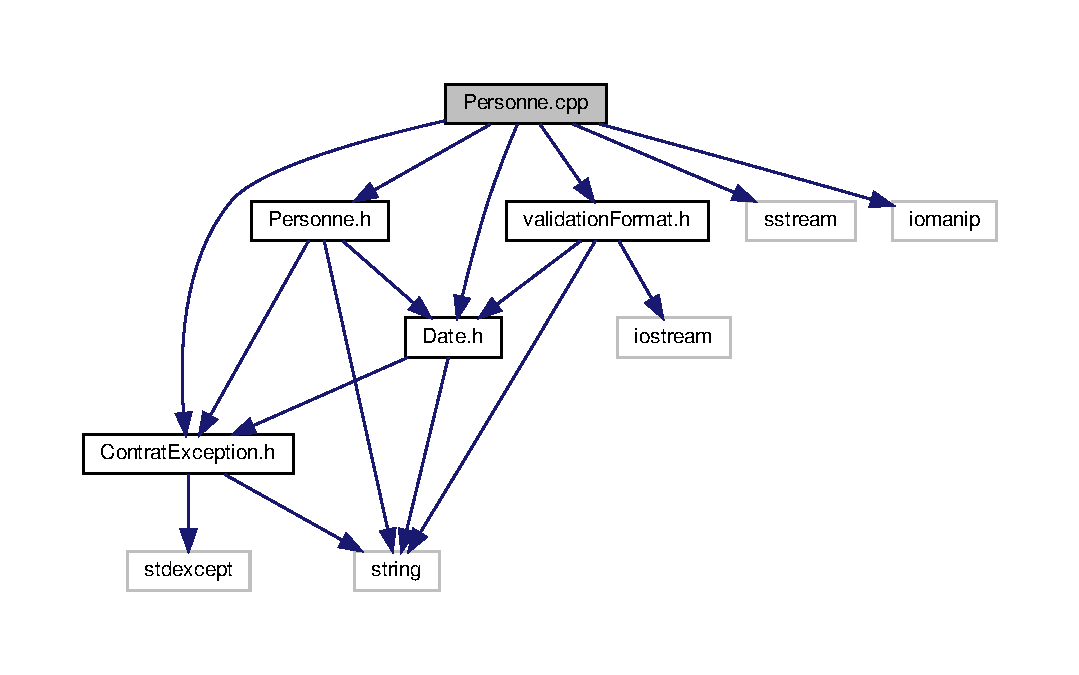
\includegraphics[width=350pt]{Personne_8cpp__incl}
\end{center}
\end{figure}


\subsection{Detailed Description}
Cette classe sert au maintien et à la manipulation des personnes. Cette classe est abstraite. 

Les valeurs qui entrent dans la classe doivent être validée à priori. 

Attributs\+: string p\+\_\+nom, string p\+\_\+prenom, Date p\+\_\+date\+Naissance, string p\+\_\+telephone \begin{DoxyAuthor}{Author}
Jordan Longval 
\end{DoxyAuthor}
